\documentclass[a4paper,12pt,titlepage,finall]{article}

\usepackage{amssymb}
\usepackage{csvsimple}
\usepackage{tikz}
\usepackage{pgfplots}
\usepackage{cmap}
\usepackage{color}
\usepackage[unicode]{hyperref}
\usepackage[utf8x]{inputenc}
\usepackage[english,russian]{babel}
\usepackage{hyperref}
\usepackage[T2A]{fontenc}
\newcommand{\gt}{\textgreater} % знак больше
\newcommand{\lt}{\textless}       % знак меньше]
\usepackage[margin=2cm]{geometry}		 % для настройки размера полей
\usepackage{indentfirst}         % для отступа в первом абзаце секции
\usepackage{amsmath}
\usepackage{fancyvrb}
\usepackage{graphicx}
\usepackage{listings}



\usepackage{listings}

\lstset{
inputencoding=utf8x,
extendedchars=false,
keepspaces = true,
language=C++,
basicstyle=\ttfamily,
keywordstyle=\color[rgb]{0,0,1},
commentstyle=\color[rgb]{0.026,0.112,0.095},
stringstyle=\color[rgb]{0.627,0.126,0.941},
numberstyle=\color[rgb]{0.205, 0.142, 0.73},
morecomment=[l][\color{magenta}]{\#},
frame=shadowbox,
escapechar=`,
numbers=left,
breaklines=true,
basicstyle=\ttfamily,
literate={\ \ }{{\ }}1,
tabsize=2,
basicstyle=\footnotesize,
}


% выбираем размер листа А4, все поля ставим по 3см
\geometry{a4paper,left=10mm,top=10mm,bottom=10mm,right=10mm}

\setcounter{secnumdepth}{0}      % отключаем нумерацию секций


\begin{document}
% Титульный лист
\begin{titlepage}
    \begin{center}
	{\small \sc Московский государственный университет \\имени М.~В.~Ломоносова\\
	Факультет вычислительной математики и кибернетики\\}
	\vfill
	{\Large \sc Компьютерный практикум по учебному курсу ""}\\
	~\\
	{\large \bf <<Введение в численные методы>> \\
	Задание 2}\\
	~\\
	{\small \bf  Числнные методы решения дифференцальных уравнений\\ }
	~\\
	{\large \bf  ОТЧЕТ \\ }
	~\\
	{\small \bf  о выполненном задании \\ }
	~\\
	{\small \sc студента 206 учебной группы факультета ВМК МГУ\\}

	{\small \sc Николайчука Артёма Константиновича\\}
	\vfill
    \end{center}

    \begin{center}
	\vfill
	{\small гор. Москва\\2020 г.}
    \end{center}
\end{titlepage}

% Автоматически генерируем оглавление на отдельной странице
\tableofcontents

\newpage

\section{Постановка задачи}

\subsection{Задача 1}
Рассматривается ОДУ первого порядка, разрешённое относительно производной, c дополнительным начальным условием в точке a и имеющее вид:
	\begin{equation*}
	\begin{cases}
	 \frac{dy}{dx} = f(x, y) &  a \leq x \leq b  \\
	 y(a) = y_{0}
	\end{cases}
	(1)
	\end{equation*}
Необходимо найти решение данной задачи Коши в предположении, что правая часть уравнения $f = f(x, y)$ гарантирует существование и единственность решения задачи Коши.\\

Рассматривается система линейных ОДУ первого порядка, разрешённых относительно производной, с дополнительными условиями в точке а:
\begin{equation*}
\begin{cases}
\frac{dy_{1}}{dx} = f_{1}(x, y_{1}, y_{2})\\
\frac{dy_{2}}{dx} = f_{2}(x, y_{1}, y_{2})
 &  a \leq x \leq b  \\
y_{1}(a) = y_{1}^{0},  y_{2}(a) = y_{2}^{0}
\end{cases}
(2)
\end{equation*}
Необходимо найти решение данной задачи Коши  в предположении, что правые части уравнений гарантируют существование и единственность решения задачи Коши для системы.

\subsection{Задача 2}
Рассматривается  краевая задача для дифференциального уравнения второго порядка с дополнительными условиями в граничных точках:
\begin{equation*}
\begin{cases}
y"+p(x)y'+q(x)y = f(x) \\
\sigma_{1}y(a) + \gamma_{1}y'(a) = \delta_{1} &  a \leq x \leq b  \\
\sigma_{2}y(b) + \gamma_{2}y'(b) = \delta_{2}
\end{cases}
(3)
\end{equation*}
Необходимо найти решение данной краевой задачи.


\newpage

\section{Цели}


\begin{itemize}

\item Часть 1

Изучить методы Рунге-Кутта второго и четвертого порядка точности, применяемые для численного решения задач Коши для дифференциального уравнения (или системы) первого порядка:

\begin{itemize}
\item Решить задачу Коши (1) или (2) наиболее известными и широко используемыми на практике методами Рунге-Кутта второго и четвертого порядка точности, аппроксимировав дифференциальную задачу соответствующей разностной схемой (на равномерной сетке); полученное конечно-разностное уравнение (или уравнения в случае системы), представляющее фактически некоторую рекуррентную формулу, просчитать численно;

\item Найти численное решение задачи и построить его график;

\item Найденное численное решение сравнить с точным решением дифференциального уравнения

\end{itemize}

\item Часть 2

Изучить метод прогонки решения краевой задачи для дифференциального уравнения второго порядка:

\begin{itemize}
\item Решить краевую задачу (3) методом конечных разностей, аппроксимировав ее разностной схемой второго порядка точности (на равномерной сетке); полученную систему конечно-разностных уравнений решить методом прогонки;

\item Найти разностное решение задачи и построить его график;

\item Найденное разностное решение сравнить с точным решением дифференциального уравнения
\end{itemize}

\end{itemize}

\newpage


\section{Описание алгоритмов}

\subsection{Метод Рунге-Кутты}
Будем использовать следующие формулы для численного решения задачи Коши, приближающие точное решение с четвёртым порядком точности относительно диаметра разбиения отрезка, на котором решается поставленная задача.\\
Положим:\\
\begin{itemize}
\item $n$ - число точек разбиения отрезка\\
\item $ h=\frac{a - b}{n}$ - диаметр разбиения отрезка\\
\item $ x_{i} = a + h * i, y_{i} = y(x_{i}), 0 \leq i \leq n $ - сетка и сеточная функция\\
\end{itemize}

Метод Рунге-Кутты 2 порядка точности для рекуррентного вычисления сеточной функции примет следующий вид:
~\\

			$y_{i + 1} = y_{i} + \frac{h}{2}(f(x_{i},y_{i}) + f(x_{i} + h, y_{i} + h * f(x_{i}, y_{i})))\\$




Метод Рунге-Кутты 4 порядка точности для рекуррентного вычисления сеточной функции примет следующий вид:
	\begin{equation*}
		\begin{cases}
			k_{1} = f(x_{i}, y_{i})\\
			k_{2} = f(x_{i} + \frac{h}{2}, y_{i} + \frac{h}{2}k_{1})\\
			k_{3} = f(x_{i} + \frac{h}{2}, y_{i} + \frac{h}{2}k_{2})\\
			k_{4} = f(x_{i} + h, y_{i} + hk_{3})\\
			y_{i + 1} = y_{i} + \frac{h}{6}(k_{1} + 2 \cdot (k_{2} + k_{3}) + k_{4})
		\end{cases}
\end{equation*}


\newpage

Для задачи (2) метод Рунге-Кутты 4 порядка для рекуррентного вычисления сеточной функции примет следующий вид:
\begin{equation*}
\begin{cases}
k_{11} = f_{1}(x_{i}, y^{i}_{1}, y^{i}_{2})\\
k_{21} = f_{2}(x_{i}, y^{i}_{1}, y^{i}_{2})\\
k_{12} = f_{1}(x_{i} + \frac{h}{2}, y^{i}_{1} + \frac{h}{2}k_{11}, y^{i}_{2} + \frac{h}{2}k_{21})\\
k_{22} = f_{2}(x_{i} + \frac{h}{2}, y^{i}_{2} + \frac{h}{2}k_{11}, y^{i}_{2} + \frac{h}{2}k_{21})\\
k_{13} = f_{1}(x_{i} + \frac{h}{2}, y^{i}_{1} + \frac{h}{2}k_{12}, y^{i}_{2} + \frac{h}{2}k_{22})\\
k_{23} = f_{2}(x_{i} + \frac{h}{2}, y^{i}_{2} + \frac{h}{2}k_{12}, y^{i}_{2} + \frac{h}{2}k_{22})\\
k_{14} = f_{1}(x_{i} + h, y^{i}_{1} + hk_{13}, y^{i}_{2} + hk_{23})\\
k_{24} = f_{2}(x_{i} + h, y^{i}_{1} + hk_{13}, y^{i}_{2} + hk_{23})\\
y^{i + 1}_{1} = y^{i}_{1} + \frac{h}{6}(k_{11} + 2 \cdot (k_{12} + k_{13}) + k_{14})\\
y^{i + 1}_{2} = y^{i}_{2} + \frac{h}{6}(k_{21} + 2 \cdot (k_{22} + k_{23}) + k_{24})
\end{cases}
\end{equation*}

\subsection{Краевая задача}
Для решения данной задачи запишем заданное дифференциальное уравнение в узлах сетки и краевые условия:\\
\begin{equation*}
\begin{cases}
y''_{i}+p_{i}y'_{i}+q_{i}y_{i}=f_{x}, x_{i} = a + i\frac{b-a}{n} & 0 \leq i \leq n\\
\sigma_{1}y_{0} + \gamma_{1}y'_{0} = \delta_{1}\\
\sigma_{2}y_{n} + \gamma_{2}y'_{n} = \delta_{2}
\end{cases}
\end{equation*}

Для $ 1 \leq i \leq n-1 $ существует следующее разностное приближение для первой и второй производной и самой сеточной функции:\\
\begin{equation*}
\begin{cases}
y''_{i}=\frac{y_{i+1}-2y_{i}+y_{i-1}}{h^{2}}\\
y'_{i}=\frac{y_{i+1}-y_{i-1}}{2h}\\
\end{cases}
\end{equation*}

В результате подстановки этих разностных отношений в начальное уравнение в виде сеточной функции получим линейную систему из n+1 уравнений с n+1 неизвестными $y_0, y_1,...,y_n$:\\
\begin{equation*}
\begin{cases}
y''_{i}=\frac{y_{i+1}-2y_{i}+y_{i-1}}{h^{2}} + p_{i}\frac{y_{i+1}-y_{i-1}}{2h} + q_{i}y_{i} = f_{i} & 1 \leq i \leq n-1\\
\sigma_{1}y_{0} + \gamma_{1}\frac{y_{0}  -y_{0}}{h}= \delta_{1}\\
\sigma_{2}y_{1} + \gamma_{2}\frac{y_{n}  -y_{n-1}}{h}= \delta_{2}
\end{cases}
\end{equation*}

\newpage

Решим полученную систему, используется метод прогонки. \\
После преобразований получим:
\begin{equation*}
\begin{cases}
C_{0}y_{0} + B_{0}y_{1}=F_{0}\\
A_{i}y_{i-1}+C_{i}y_{i} + B_{i}y_{i+1}=F_{i} & 1 \leq i \leq n-1 \\
A_{n}y_{n-1} + C_{n}y_{n}=F_{n}
\end{cases}
\end{equation*}

\bigskip
\begin{minipage}{\linewidth}
\begin{equation*}
\begin{cases}
\alpha_{0}=-\frac{B_{0}}{C_{0}}\\
\beta_{0}=\frac{F_{0}}{C_{0}}\\
\alpha_{i}=-\frac{B_{i}}{C_{i} + A_{i}\alpha_{i-1}}\\
& 1 \leq i \leq n-1\\
\beta_{i}=\frac{F_{i} - A_{i}\beta_{i-1}}{C_{i} + A_{i}\alpha_{i-1}}\\
\\
y_{n}=\frac{F_{n} - A_{n}\beta_{n-1}}{C_{n} + A_{n}\alpha_{n-1}}\\
y_{i}=\beta_{i}+\alpha_{i} *y_{i+1} & 0 \leq i \leq n-1
\end{cases}
\end{equation*}
\end{minipage}
Откуда и находим все $y_{i}$
\newpage

\section{Тестировние функций}
\subsection{Тест1}
\begin{equation*}
 \begin{cases}
   y' = -y - x^{2}\\
   x_0 = 0\\
   y_0 = 10\\
 \end{cases}
\end{equation*}
Точное решение: $y = -x^2 + 2x - 2 + 12 e^{-x} $\newline

Ошибка метода второго порядка при 10 шагах $z_2 = 10^{-3}$, метода четвёртого порядка $z_4 = 4 \cdot 10^{-6}$

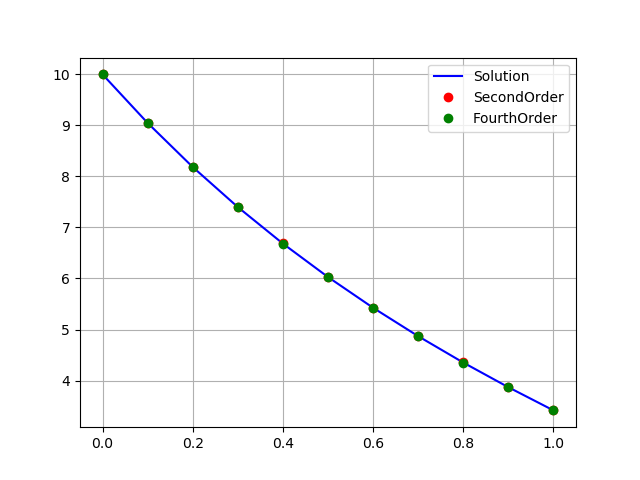
\includegraphics[width=450pt]{Graphics/0.0.png}\newline
\newpage
\subsection{Тест2}
\begin{equation*}
 \begin{cases}
   y' = y + 2x - 3\\
   x_0 = 0\\
   y_0 = 2\\
 \end{cases}
\end{equation*}
Точное решение: $y = 1 + e^{x} - 2x$\newline

Ошибка метода второго порядка при 30 шагах $z_2 = 10^{-4}$, метода четвёртого порядка $z_4 = 10^{-8}$

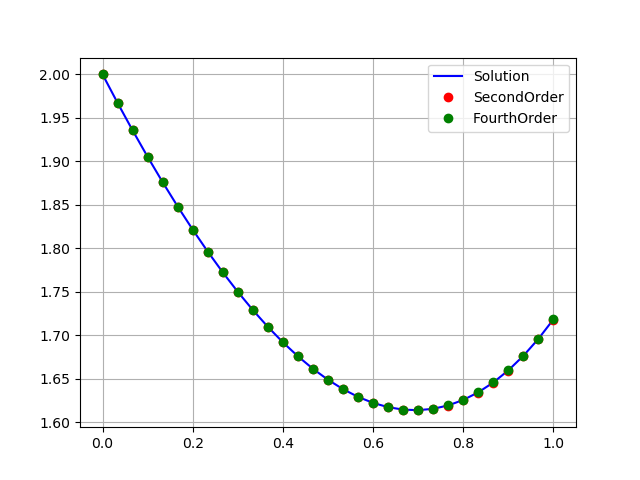
\includegraphics[width=450pt]{Graphics/0.1.png}\newline
\newpage
\subsection{Тест3}
\begin{equation*}
 \begin{cases}
   x' = \sqrt{t^2 + 0.1x^2} + y\\
   y' = \cos{(2.1y)} + x\\
   x_0 = 0.5\\
   y_0 = 1\\
   t \in [0, 1]\\
 \end{cases}
\end{equation*}
Аналитического решения не существует\newline

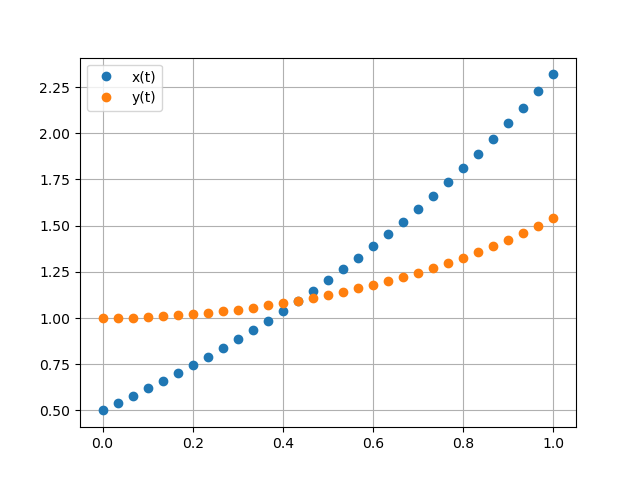
\includegraphics[width=450pt]{Graphics/1.0.png}\newline
\newpage
\subsection{Тест4}
\begin{equation*}
 \begin{cases}
   x' = 3x - y\\
   y' = 4x - y\\
   x_0 = 1\\
   y_0 = 1\\
   t \in [0, 1]\\
 \end{cases}
\end{equation*}
Аналитического решение:\newline
\begin{equation*}
 \begin{cases}
   x = (1 + t) \cdot e^{t}\\
   y = (1 + 2t) \cdot e^{t}\\
 \end{cases}
\end{equation*}

Ошибка метода при 30 шагах у функции $x(t) z_x = 10^{-8}$, у функции $y(t) z_y = 10^{-7}$

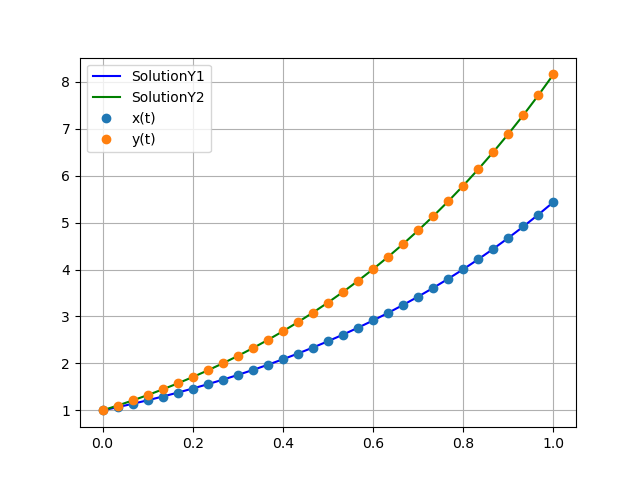
\includegraphics[width=450pt]{Graphics/1.1.png}\newline
\newpage
\subsection{Тест5}
\begin{equation*}
 \begin{cases}
   y'' - y' = 0\\
   y(0) = -1\\
   -y(1) + y'(1) = 2\\
 \end{cases}
\end{equation*}
Аналитического решение: $y = -2 + e^{x}$\\

Ошибка метода при 60 шагах $z = 0.01658$

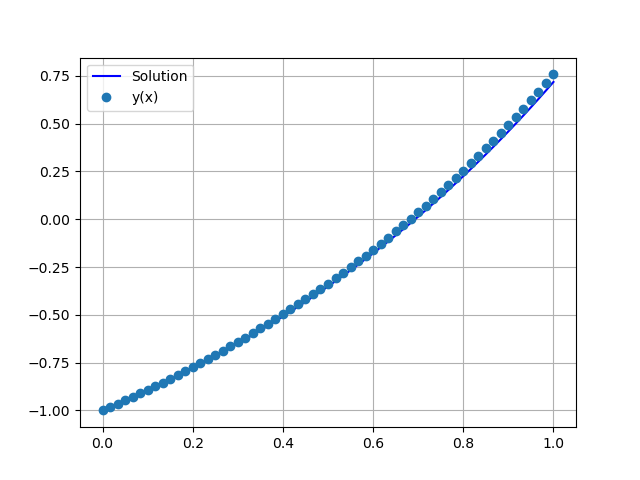
\includegraphics[width=450pt]{Graphics/2.1.png}\newline
\newpage
\subsection{Тест6}
\begin{equation*}
 \begin{cases}
   y'' + y = 1\\
   y(0) = 0\\
   y(\frac{\pi}{2}) = 0\\
 \end{cases}
\end{equation*}
Аналитического решение: $y = 1 - \sin{x} - \cos{x}$\\

Ошибка метода при 30 шагах $z = 5 \cdot 10^{-5}$

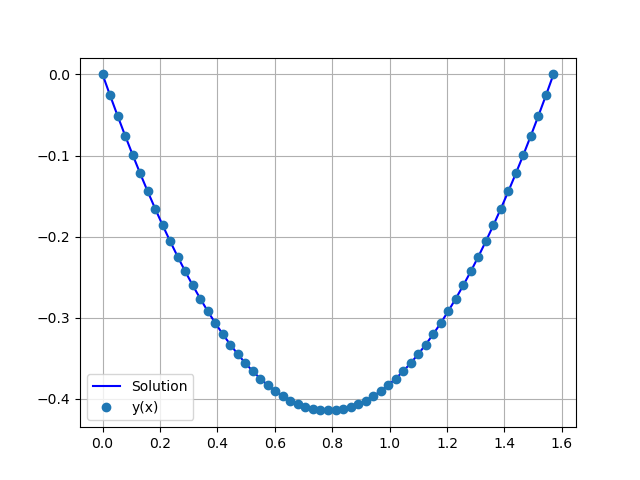
\includegraphics[width=450pt]{Graphics/2.2.png}\newline
\newpage
\subsection{Тест7}
\begin{equation*}
 \begin{cases}
   y'' - 3xy + 2y = 1.5\\
   y'(0.7) = 1.3\\
   0.5 \cdot y(1) + y'(1) = 2\\
 \end{cases}
\end{equation*}
Аналитического решения не существует\\

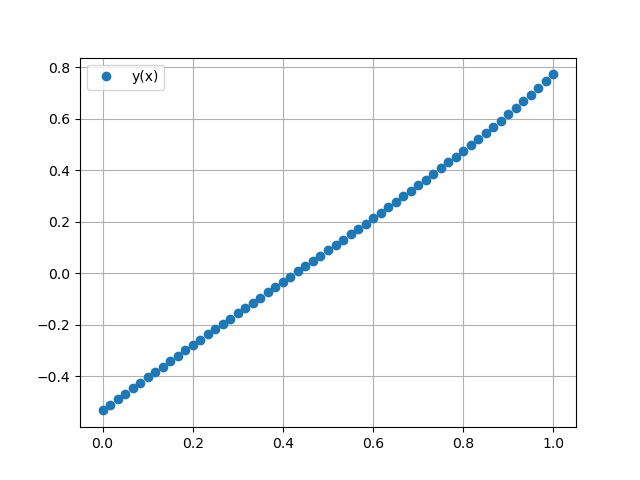
\includegraphics[width=450pt]{Graphics/2.0.png}\newline
\newpage
\section{Исходный код} Исходный код проекта размещён на гитхабе \href{https://github.com/Strannik2001/Computing_Methods}{https://github.com/Strannik2001/Computing\_Methods}\\
\newpage
\end{document}